\chapter{Fluid Structure Interaction Problem}
So far I have introduced the fluid and solid equations, and the descriptions in which they are stated. In this chapter I will introduce the full FSI problem. With all the equations, conditions and discretization needed to to build a solver. \newline

When we compute FSI problems the computing domain is split into three parts, Fluid, Structure and Interface. Fluid and structure domains are as we know separated, and different constitutive equations are solved in each domain. The place in which fluid and structure meet is what we call the interface. The manner in which we treat the interface gives the two main methods for solving FSI problems \cite{Liu2014}. The first method is called fully Eulerian. In fully Eulerian both the fluid and structure equations are solved in an Eulerian description. Here the interface is tracked across a still standing domain \cite{Valkov2015}. The fully Eulerian description is suited for fluid problems but is problematic for structure problems and certainly FSI where tracking of the interface across the domain is a difficult task. I therefore introduce the more commonly used method ALE. Which is the method that will be used in this thesis. \newline

ALE stands for Arbitrary Lagrangian Eulerian. The ALE method entails formulating the fluid equations in an Eulerian framework and the solid in a Lagrangian framework. The entire domain itself moves with the structural displacements and the fluid moves through these points. In the ALE framework we get best of both world. The structure equation will remain as previously stated \eqref{eq:Solid}, and we will need to change the fluid equations to take into account the moving domain changing the fluid velocity. Dealing with the movement of the domain is done in two ways. One way is to move the domain itself in relation to the structural displacements, and use this new domain to calculate the equations every time.
Moving the domain gives advantages as we can explicitly represent the fluid-structure interface, and the equations are stated in a more familiar manner. But problems arise when there are large deformations in the solid giving large deformations into the fluid domain. Moving the mesh with large deformation can be a challenge. \newline

In this thesis the ALE approach is used from a reference frame.
Meaning we solve the equations on a initial, stress free domain, and use a series of mappings to account for the movements of the domain. The equations are mapped to the current domain, that is where the domain has moved to in the present time. It is the displacements in the solid that determines the mappings. The displacements in the solid and the interface are extrapolated into the fluid mesh. I will deal with the manner in which these extrapolations work in this chapter. \newline

From a technical point of view, both moving the mesh and using a reference frame are equivalent \cite{Richter2016}. Since the reference frame method does not need a function to move the mesh between each time iteration can be less time consuming. The interface is also located in the same position, making the interface easy to track. \newline

Lastly in this chapter the equations are discretized. Discretization of the equations is tackled using either a monolithic or a partitioned approach. We will go into details later, but the overall idea is that a monolithic scheme involves computing all the equations together into one block, while the partitioned splits up into parts. That is we solve the fluid problem and structure problem separately. The advantage of this is that we can use existing solvers and techniques for each of the problems, but the difficulty is the treatment of the interface. The monolithic approach however, offers more stability but is more costly as the size of the problem increases\cite{Liu2014}. \newline

I will start by introducing the mappings, this follows the notation and ideas from \cite{Richter2016}:

\section{Mapping between different frames of reference}
\begin{figure}[H]
\label{pic:FSI_mapping}
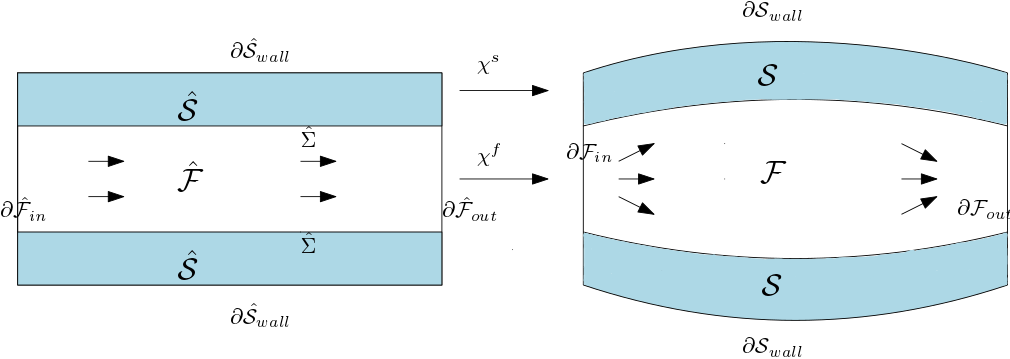
\includegraphics[scale=0.45]{./FSI_ALE_formulation/FSI_mapping.png}
\caption{Mapping of domain from reference to current}
\end{figure}

Let $\hat{\mathcal{V}}$ be a reference volume and $\mathcal{V}(t)$ be the current time volume. Then using \eqref{eq:deformation_gradient} and \eqref{eq:J} we define a mapping between the volumes from the current to reference configurations:

\begin{equation}
 \int_{\mathcal{V}(t)} 1  dx = \int_{\hat{\mathcal{V}}} J dx  
\end{equation}

The gradients acting on a vector $ \bold{u} $ will also be mapped between current and reference configurations:

\begin{equation}
\int_{\mathcal{V}(t)} \nabla \bold{u}   dx = \int_{\hat{\mathcal{V}}} J  \nabla \bold{u}F^{-1} dx  
\end{equation}

Same for the divergence of a vector $ \bold{u}$:

\begin{equation}
\int_{\mathcal{V}(t)} \nabla \cdot \bold{u}   dx = \int_{\hat{\mathcal{V}}} \nabla \cdot( J  F^{-1} \bold{u}) dx  
\end{equation}

\section{Governing equations for Fluid Structure Interaction}

We will formulate the equations in the Eulerian, Lagrangian and the ALE description. We start by briefly talking about time derivatives in the different configurations. In the Lagrangian setting the total and partial derivatives are the same \cite{Wick2011}:

\subsection{Derivatives in different frameworks}
\begin{equation}
D_t f(x,t) = \partial_t f(x,t)
\end{equation}

in the Eulerian framework we have the following relation between total and partial derivatives:

\begin{equation}
D_t f(x,t) = \bold{u} + \partial_t f(x,t)
\end{equation}

whilst in the ALE framework we extend this concept to take into account the motion of the domain:

\begin{equation}
D_t f(x,t) = \bold{w} + \partial_t f(x,t)
\end{equation}

Here we can see that for the Lagrangian framework $ \bold{w}$ is zero and for Eulerian $\bold{w} = \bold{u}$.

\subsection{Solid equation}
We express the solid balance laws in the Lagrangian formulation from the initial configuration

\begin{equation}
\rho_s \frac{\partial \bold{u}}{\partial t} = \nabla \cdot (P) \hspace{4mm}in\hspace{4mm} \hat{\mathcal{S}} 
\end{equation}

\subsection{Fluid equations}


The fluid domain is moving, and therefore we need to redefine the velocity in the convective term in \eqref{eq:NS} to account for the moving domain 
\begin{equation}
\bold{u} \cdot \nabla \bold{u} \rightarrow (\bold{u}-\frac{\partial d_f}{\partial t}) \cdot \nabla \bold{u}  
\end{equation}
where $d_f$ is the deformation in the fluid domain. We see that $\bold{w}$ is written as $\frac{\partial d}{\partial t}$ . Now the actual fluid velocity will be $u-\frac{\partial d}{\partial t}$ 

The fluid equations are denoted from the initial configuration using the aforementioned mappings:

\begin{align}
\int_{\mathcal{V}(t)} \rho_f \frac{\partial \bold{u}}{\partial t} dx & = \int_{\hat{\mathcal{V}}}  \rho_f J \frac{\partial \bold{u}}{\partial t} dx \\
\int_{\mathcal{V}(t)} \nabla \bold{u} (\bold{u}-\frac{\partial d}{\partial t}) dx  &= \int_{\hat{\mathcal{V}}} ((\nabla \bold{u})F^{-1}(\bold{u}-\frac{\partial d}{\partial t}) dx  \\
\int_{\mathcal{V}(t)} \nabla \cdot \bold{u} dx  &=\int_{\hat{\mathcal{V}}}  \nabla \cdot (J F^{-1} \bold{u}  ) dx \\
\int_{\mathcal{V}(t)} \nabla \cdot \sigma_f dx &= \int_{\hat{\mathcal{V}}} \nabla \cdot( J F^{-1} \hat{\sigma_f} )     dx \\
\hat{\sigma_f} &= -pI + \mu ( \nabla \bold{u} F^{-1} + F^{-T} \bold{u}^{T}  ) 
\end{align}

Assembling all these terms together with \eqref{eq:NS} gives the fluid equations from a reference frame:

\begin{align}
\label{eq:NS_mapped}
\rho_f J \big( \frac{\partial \bold{u}}{\partial t} dx + (\nabla \bold{u})F^{-1}(\bold{u}-\frac{\partial d}{\partial t}) \big) &= \nabla \cdot( J F^{-1} \hat{\sigma_f} ) + J \rho_f f \\
\nabla \cdot (J F^{-1} \bold{u} ) &= 0
\end{align} 

\section{Mesh motion techniques} \label{sec:meshmotion}
Using the ALE method the deformations from the structure through the interface is extrapolated to the fluid domain. The fluid domain itself acts as a structure, deforming according to the deformations from the structure domain.
The choice of mesh motion technique is important for the overall FSI problem to be calculated \cite{Wick2011a}. When large deformations occur, we need a good lifting operator to uphold the integrity of the computing domain. A poor choice will make the mesh overlap and singularities may occur. I will in this section present different mesh motion techniques, that act differently on the computational domain. In \ref{sec:mesh_motion} the techniques will be tested and investigated.

\subsection{Harmonic extension}
For small to moderate deformations we can use a harmonic extension to lift the deformations. The harmonic extenstion uses the Laplace equation, transporting the deformations from the solid into the fluid domain. A variable $\alpha_u > 0$ can be multiplied to the Laplace equation, to control the amount of lifting of deformations to the fluid domain.

\begin{align}
 - \alpha_u \nabla^2 d =& 0\hspace{4mm} in \hspace{2mm} \hat{\mathcal{F}}\\
  \hspace{4mm} d =& 0 \hspace{4mm } on \hspace{2mm }  \partial \hat{\mathcal{F}} / \hat{\Sigma}
\end{align}

When using the harmonic lifting operator the variable $\alpha_u$ is very important when calculating moderate deformations. For small deformations a constant can be used for $\alpha_u$. But for larger deformations we need to be a bit more clever. A good strategy for choosing $\alpha_u$ is proposed by Wick in \cite{Wick2011a}, and further discussed in \cite{Stein2003}. Which is an alpha that gets bigger when closer to the interface. This is a smart choice since this upholds the cell structure closer to the interface where most of the cell distortion appears. 

\subsection{Linear elastic extension}
Since the fluid domain acts as structure we can use a linear elastic equation to lift the deformations from the solid into the fluid domain. The linear elastic equation is best known from computing solid problems \cite{Wick2011a}.  The model is as follows:

\begin{align}
-\nabla \cdot \sigma_{mesh} &= 0 \hspace{4mm} in \hspace{2mm} \hat{\mathcal{F}}\\
\hspace{4mm} d &= 0 \hspace{4mm } on \hspace{2mm }  \partial \hat{\mathcal{F}} / \hat{\Sigma} \\
\sigma_{mesh} &= \alpha_\lambda (tr\epsilon)I + 2\alpha_\mu \epsilon 
\end{align}
where $\epsilon = \frac{1}{2}(\nabla d + (\nabla d)^T)$. $\epsilon$ is the linearized version of the strain tensor \eqref{eq:StrainTensor}. The parameters $\alpha_\lambda$ and $\alpha_\mu$ are chosen to uphold domain quality. This is done by computing the parameters $\alpha_\lambda$ and $\alpha_\mu$ from Youngs modulus and poisson ration. 

\subsection{Biharmonic extension} 
The last extension is the biharmonic extension. The biharmonic extension provides more freedom than the harmonic and linear elastic in choosing boundary conditions and choice of parameter $\alpha_u > 0$. This is because the biharmonic extension, extends the deformation in a manner that upholds the integrity of the cells even in large deformations, even with $\alpha_u$ as a constant. In its simplest form it is written as:

\begin{equation}
- \alpha_u \nabla^4 d = 0 \hspace{4mm}  in \hspace{2mm} \hat{\mathcal{F}}\\
\end{equation}

The biharmonic extension is calculated with a mixed formulation where we introduce a new function $\omega$ (not to be confused with the deformation velocity), this function is added to the system so that we solve for 4 functions:

\begin{equation}
\omega = \alpha_u \nabla^2 d \hspace{4mm} and \hspace{4mm} - \alpha_u \nabla^2 \omega = 0 \hspace{2mm}   in \hspace{2mm} \hat{\mathcal{F}}
\end{equation}
with the two types of boundary conditions. The first being:
\begin{equation}
d = \partial_n d = 0 \hspace{4mm} on \hspace{2mm} \partial \hat{\mathcal{F}} \hspace{2mm} \textbackslash \hspace{2mm} \hat{\Sigma}
\end{equation}

The second imposes conditions on the function $\omega$, and are written in terms of single component functions $d^{(1)},d^{(2)}$ and $\omega^{(1)}, \omega^{(2)}$	
\begin{align}
d^{(1)} =& \partial_n d^{(1)} = 0 , and \hspace{4mm}   \omega^{(1)} = \partial_n \omega^{(1)} = 0    \hspace{4mm} on \hspace{2mm} \partial \hat{\mathcal{F}}_{in,out} \\
d^{(2)} =& \partial_n d^{(2)} = 0 , and \hspace{4mm}   \omega^{(2)} = \partial_n \omega^{(2)} = 0    \hspace{4mm} on \hspace{2mm} \partial \hat{\mathcal{F}}_{walls} \\
\end{align}

Since the biharmonic extension is of fourth order character it will have a higher computational cost \cite{Richter2016} than the harmonic or linear elastic. 


\section{Coupled Fluid Structure Interface conditions}
In figure \ref{pic:FSI_mapping} we see a typical Fluid Structure Interaction. The fluid is surrounded by elastic walls, like a blood vessel. The inflow at $\partial \hat{\mathcal{F}}_{in}$, a change in pressure, or a motion of the solid determines the flow of the fluid.
The fluid`s stress on the walls causes deformation in the solid domain and vice versa. The interface is where these energies are transferred and we therefore need conditions on the interface. \newline

Let $\Omega \in \hat{\mathcal{S}} \cup \hat{\mathcal{F}} $ be a global domain that is made up of the fluid, structure, and the interface. We define a global velocity function $u$ that describes the fluid velocity in the fluid domain and the structure velocity in the structure domain. Using a global velocity makes the velocity continuous across the entire domain. Let interface be $ \hat{\Sigma} \in \hat{\mathcal{S}} \cap \hat{\mathcal{F}}  $.\newline 
The three interface comes from simple physical properties and consist of \cite{Richter2016}:

\begin{itemize}
\item \textit{Kinematic condition}: $\bold{u}_f = \bold{u}_s  \hspace{2mm} on \hspace{2mm} \hat{\Sigma}$. The fluid and structure velocities are equal on the interface. Meaning the fluid moves with the interface at all times. \\
Since we use a global function for $\bold{u}$ in both fluid and structure domains, this condition is upheld.\\ 
The fluid and solid velocities are usually in different coordinate systems, the solid velocity is then not available in Eulerian Coordinates. We instead link fluid velocity at the interface by using the fact that $\bold{u}_s = \frac{\partial d}{\partial t}$. Setting $\bold{u}_f = \frac{\partial d}{\partial t}$ at the interface.

\item \textit{Dynamic condition}: $  \sigma_f n_f = \sigma_s n_s \hspace{2mm} on  \hspace{2mm}\hat{\Sigma}   $. \\
	This relates to Newtons third law of action and reaction. The forces on the interface area, here written as the normal stresses are balanced on the interface. These will be written in a Lagrangian formulation: \\
	$J\sigma_f F^{-T} n_f = P n_s \hspace{2mm} on  \hspace{2mm}\hat{\Sigma} $. \\
	The dynamic condition is a Neumann condition that belongs to both subproblems.
	
\item \textit{Geometrical condition}: This condition says that the fluid and structure domains do not overlap, but rather that elements connect so the functions needing to transfer force are continuos across the entire domain.
\end{itemize}

\section{Monolithic FSI Problem}
As stated in the introduction there are generally two types of schemes used when simulating FSI. The first is the partitioned approach where fluid and structure are solved sequentially.  This approach is appealing in that we have a wealth of knowledge and techniques on how to solve each of these kinds of problems in an efficient manner. The difficulty however is dealing with the interface. As we know there are kinematic and dynamic conditions needed in FSI, and the coupling of these conditions is where the problems arise. So called explicit coupled schemes are known to be unconditionally unstable for standard Dirichlet-Neumann strategies when there is a large amount of added-mass in the system \cite{Fernandez2015}, \cite{VanBrummelen2009}. There are however, schemes which offer added-mass free stability with explicit coupling, where the interface is treated through a Robin-Neumann coupling. First for a coupling with a thin walled structure \cite{Fernandez2013} and later with an extension to thick wall \cite{Fernandez2015}. These schemes are rather complex and uses a number of techniques that are out of the scope of this thesis. ( This may be in more detail in a later chapter (discussion and further work.) ) \newline

The other approach is  called monolithic. In the monolithic approach all of the equations are solved at once. This approach has the advantage of offering numerical stability for problems with strong added-mass effects \cite{Liu2014}, and are fully coupled. The disadvantage over the partitioned approach is that we loose flexibility when solving many equations simultaneously, and the problems can quickly become large and computationally costly. \newline

\begin{comment}
We start by stating the entire FSI ALE problem in a monolithic framework using the mapped approach: 

Find $\bold{u} \in \hat{\mathcal{F}} , p \in \hat{\mathcal{F}} \text{  and  } d \in \hat{\mathcal{S}} \text{  such that}:$ 
\begin{align}
\rho_f J \big( \frac{\partial u}{\partial t} + (\nabla \bold{u} )F^{-1}(\bold{u} -\frac{\partial d}{\partial t})\big)  + \nabla \cdot( J \hat{\sigma_f} F^{-T})  &= 0 \hspace{8mm}\text{on  } \hat{\mathcal{F}} \\
\nabla \cdot (J \bold{u}  F^{-T})\big) &= 0 \hspace{8mm} \text{on  } \hat{\mathcal{F}}   \\
\rho_s \frac{\partial \bold{u} }{\partial t} + \nabla \cdot F S_s,&=0 \hspace{8mm} \text{on  } \hat{\mathcal{S}}\\
\nabla^2 d &= 0 \hspace{8mm} \text{on  } \hat{\mathcal{F}}\\
\bold{u} - \frac{\partial d}{\partial t}  &= 0 \hspace{8mm} \text{on  } \hat{\mathcal{S}}\\
J\sigma_f F^{-T} n_f &= \sigma_s  n_s \hspace{3mm} \text{on  } \hat{\Sigma}
\end{align}
\end{comment}

\section{Discretization of monolithic FSI equations}\label{Discretization}
After introducing all the equations and boundary conditions needed to solve a FSI problem. We are ready to discretize the equations into one monolithic scheme. The equations will be discretized and solved using finite difference and finite element methods. I will introduce a so called $\theta$-scheme which will make it easy to implement different schemes, by choosing a value for $\theta$.
I will briefly introduce the spaces needed to discretize, following the ideas and notations of \cite{Wick2011}:

\subsubsection{Spaces}
Let $ X \in \mathbb{R}^d , d \in\{ 1,2  \} $ be a time dependent domain we define:

\begin{equation}
\hat{V}_X := H^1(X), \hspace{6mm}  \hat{V}^1_X := H^1_0(X) 
\end{equation}

$ H^1 $ indicating a Hilbert space and

\begin{equation}
\hat{L}_X := L^2(X), \hspace{6mm} \hat{L}^0_X := L^2(X) / \mathbb{R}
\end{equation}

$L^2$ indicating a standard Lebesque space.

The trial and test spaces for the velocity variable in the fluid domain,

\begin{equation}
\hat{V}^0_{f,u} := \{ \hat{u} \in H^1_0(\mathcal{F}) : \hat{u}_f = \hat{u}_s \hspace{2mm} on \hspace{2mm} \hat{\Sigma}  \}
\end{equation}

and the same for the artificial displacement in the moving fluid domain:

\begin{equation}
\hat{V}^0_{f,d} := \{ \hat{d} \in H^1_0(\mathcal{F}) : \hat{d}_f = \hat{d}_s \hspace{2mm} on \hspace{2mm} \hat{\Sigma}  \}
\end{equation}
\begin{equation}
\hat{V}^0_{f,d} := \{ \hat{d} \in H^1_0(\mathcal{F}) : \hat{\psi_f} = \hat{\psi_s} \hspace{2mm} on \hspace{2mm} \hat{\Sigma}  \}
\end{equation}

Now that the spaces have been defined we are ready to discretize. The temporal discretization is done using finite difference schemes and the spatial is treated with the finite element method. I will employ a $\theta-$ scheme that will enables us to easily switch between schemes.

\subsubsection{Discretization}

In the domain $\Omega$ and time interval [0,T]:

Find $ U = \{\bold{u}, d, p\} \in \hat{X}^0_D $ where $ \hat{X}^0_D := \{ \bold{u}^D_f + \hat{V}^0_{f,\bold{u}} \} \times \hat{L}_f \times \{ d_f^D + \hat{V}^0_{f,\hat{f}} \} \times \{ d_f^D + \hat{V}^0_{f,\hat{f}} \} \times \hat{L}^0_f \times \hat{L}^0_s  $ such that:

\begin{equation}
\int_0^T A(U)(\Psi) dt = \int_0^T \hat{F}(\Psi) dt \hspace{4mm} \forall  \Psi \in \hat{X}
\end{equation}

where $ \Psi = \{\phi, \psi, \gamma \} $% \hat{\psi}^\bold{u}_f, \hat{\psi}^\bold{u}_s, \hat{\psi}^d_f, \hat{\psi}^d_s, \hat{\psi}^p_f,\hat{\psi}^p_f  \}$ and

 $\hat{X} = \hat{V}^0_{f,\bold{u}} \times \hat{L}_f \times \hat{V}^0_{f,d,\hat{\Sigma}} \times \hat{V}_s^0 \times \hat{L}_f^0 \times \hat{L}_s^0  $


I first introduce the scheme using, for simplicity, the harmonic mesh motion. Let $\bold{u}$ be a global function in the entire domain instead of $\bold{u}_f$ in the fluid and $\bold{u}_s$ in the solid. Same for the test functions. This is done for ease of reading and also for the ease of implementation later.

\textbf{The full monolithic FSI variational form reads}:
\begin{align}
A(U)&= (J \rho_f \partial_t \bold{u} , \phi ) - (J (\nabla u)F^{-1}(\bold{u} - \partial_t d) , \phi )_{\mathcal{\hat{F}}}  \\
       &+ ( J \sigma_{f} F^{-T} , \nabla \phi )_{\mathcal{\hat{F}}} \\
       &+ (\rho_s \partial_t \bold{u} , \phi)_{\mathcal{\hat{S}}}   + \big(F S_s, \nabla \phi \big)_{\mathcal{\hat{S}}} \\
       &+ ( \alpha_u \nabla \bold{u}, \nabla \psi)_{\mathcal{\hat{F}}} + (\nabla \cdot (J F^{-1} \bold{u}),\gamma )_{\mathcal{\hat{F}}} \\
       \label{eq:condition}
       &+ \delta\big((\partial_t \bold{d} , \psi)_{\mathcal{\hat{S}}}  - ( \bold{u} , \psi )_{\mathcal{\hat{S}}}\big) \\ 
       &+  \big( J \sigma_{f,p} F^{-T}, \nabla \phi  \big) 	 		
\end{align}

The condition \eqref{eq:condition} , is weighted with a $\delta$ value. This is a critical detail for the program (detailed later) to run. The only two places where we use the test function $\psi$ is on this condition and the lifting operator. The weighting says in a weak manner that this condition is important for the overall program. \newline

I will here formulate the \textit{One step-$\theta$ scheme} from \cite{Wick2011}. This $\theta$ scheme has the advantage of easily being changed from the backward (implicit), forward(excplicit) or Crank-Nicholson (implicit) scheme. The Crank-Nicholson scheme is of second order, but suffers from instabilities in this monolithic scheme \cite{Wick2011}. A remedy for these instabilities is to chose a Crank-Nicholson scheme that is shifted towards the implicit side. How this is done will become evident once the scheme is defined.

We define the variational form by dividing into four categories, this may seem strenuous at first but the need for it will become evident when implementing the $\theta$-scheme. The four divided categories consists of: a time term, implicit, pressure and the rest (stress, convection):

\begin{align}
A_T(U) &= (J \rho_f \partial_t \bold{u} , \phi ) - (J (\nabla u)F^{-1}(\partial_t \bold{d}) , \phi )_{\mathcal{\hat{F}}} \\
	    & + (\rho_s \partial_t \bold{u} , \phi)_{\mathcal{\hat{S}}} + (\partial_t \bold{d} , \psi)_{\mathcal{\hat{S}}}  \\
A_I(U) &= ( \alpha_u \nabla \bold{u}, \nabla \psi)_{\mathcal{\hat{F}}} + (\nabla \cdot (J F^{-1} \bold{u}), \gamma)_{\mathcal{\hat{F}}} \\
A_E(U) &= (J (\nabla u)F^{-1} \bold{u} , \phi )_{\mathcal{\hat{F}}} + ( J \sigma_{f,u} F^{-T} , \nabla \phi )_{\mathcal{\hat{F}}} \\
	    & + \big(F S_s, \nabla \phi \big)_{\mathcal{\hat{S}}} - ( \bold{u} , \psi )_{\mathcal{\hat{S}}} \\
A_P(U) &= \big( J \sigma_{f,p} F^{-T}, \nabla \phi  \big)  	 		
\end{align}

Notice that the stress tensors have been split into a velocity and pressure part. 
\begin{align}
\sigma_{f,u} &= \mu ( \nabla u F^{-1} + F^{-T} \nabla u) \\
\sigma_{f,p} &= -p I
\end{align}

For the time group, discretization is done in the following way:
\begin{align}
A_T(U^{n,k}) \approx & \frac{1}{k} \big( \rho_f J^{n,\theta} (\bold{u}^n - \bold{u}^{n-1}) , \phi  \big)_{\mathcal{\hat{F}}} - \frac{1}{k} \big( \rho_f (\nabla u ) (\bold{d}^n - \bold{d}^{n-1}) , \phi \big)_{\mathcal{\hat{F}}} \\
+ & \frac{1}{k} \big( \rho_s  (\bold{u}^n - \bold{u}^{n-1}) , \phi  \big)_{\mathcal{\hat{S}}} +  \frac{1}{k} \big( (\bold{d}^n - \bold{d}^{n-1}) , \psi  \big)_{\mathcal{\hat{S}}}
\end{align}
And the Jacobian is written with superscript $\theta$ as:

\begin{equation}
J^{n, \theta} = \theta J^n + (1-\theta)J^{n-1}
\end{equation}

We can now introduce the \textit{One step-$\theta$ scheme}: 
Find $U^n = \{\bold{u}^n , \bold{d}^n, p^n \}$

\begin{align}
& A_T(U^{n,k}) + \theta A_E(U^{n}) + A_P(U^{n}) + A_I(U^{n}) = \\
& - (1-\theta) A_E(U^{n-1}) + \theta \hat{f}^n + (1-\theta) \hat{f}^{n-1}  
\end{align}

We notice that the scheme is selected by the choice of $\theta $. By choosing $ \theta = 1$ we get the back Euler scheme, for $ \theta = \frac{1}{2}$ we get the Crank-Nicholson scheme and for the shifted Crank-Nicholson we set $ \theta = \frac{1}{2} + k$, effectively shifting the scheme towards the implicit side. $\hat{f}$ is the body forces which will be ignored in this thesis. The shifting toward the implicit side is important for long term stability for certain time step values \cite{Wick2011}. The shifting will be investigated in the next chapter.







\subsection{Spaces and Elements}
The velocity and pressure copling in the fluid domain must satisfy the inf-sup condition. If not stabilization has to added. We here need to define some spaces that will have these desired properties.
We denote $u_h \in V_h$ and $ d_h \in W_h $, here the finite element pair og pressure and velocity mush satisfy the inf-sup condition given in ALE coordinates:
$$   \inf_{\substack{p_h \in L_{h,f}}}  \sup_{\substack{v_h \in V_{h,f}}} \frac{ (p_h, div(J_f F_f^{-1} u_h))_{\mathcal{F}} }{ \|\|J^{\frac{1}{2}} p_h  \|\|_{\mathcal{F}} \|\|  J^{\frac{1}{2}}_{f} \nabla u_h F_f^{-T} \|\|_{\mathcal{F}}  } \geq \hat{\Sigma}     $$
A good choice of spaces will be P2-P2-P1 for velocity, displacement and fluid pressure respectively. 








